\section{Material Design}
% Because we want our app to look decent, our path will be guided by material design.
Because the application should look decent, some guidelines have to be chosen and followed.
There exists frameworks and libraries with guidelines like Bootstrap\cite{bootstrap}, React\cite{react} or Material Design\cite{material}.
Bootstrap is a framework with it's own guidelines used for web development.
React is a JavaScript library that recommends Web Content Accessibility Guidelines\cite{wcag} and is also used for web development.
Material Design is a set of guidelines for developing websites, but also for Android and iOS applications.
The only one of those guidelines, that specializes on Android, is Material Design.
Google itself states: \textit{Not only should you follow material design guidelines for visual and navigation patterns, but you should also follow quality guidelines for compatibility, performance, security, and more.}\cite{design}
\todo[inline]{Why not bootstrap? Why not vue.js? First, describe and compare the possibilities, then explain why you chose what you chose}
Material design describes individual components, when to use them and when to not use them.
The description includes proportions, behaviour and color system.

\section{The three main screens}
% From specifications, it's clear that we need at least one screen for execution history, one for pipelines and one for settings.
Based on the analysis of the user requirements in \autoref{chap:requirementsengineering}, three screens which cover the functionality of displaying execution history, pipeline list and settings have to be designed.
\todo[inline]{do not say "it's clear". It isn't. "Based on the analysis of the user requirements, we will design three screens which cover the functionality..."}

\subsection{Main navigation}
On the android platform, there are multiple navigation designs and they will be described in this section.

\subsubsection{Navigation drawer}
The hamburger icon at the top left and sliding menu from left to the right is what navigation drawer looks like.
This navigation is suitable for five or more top level screens, or some sort of hierarchical menu.\cite{materialandroid}

\subsubsection{Tabs}
Slidable tabs on top of the screen.
Recommendation for this type of navigation is having at least two screens.\cite{materialandroid}
Users can click on tab names or just slide left or right in order to navigate between the screens.

\subsubsection{Bottom navigation}
Bottom navigation consists of icons, usually with text, located at the bottom of the screen.

\subsection{Conclusion about the main navigation}
The navigation drawer will not be used, because our application doesn't require five or more main screens nor a hierarchical menu.
Also, with the increasing sizes of mobile phones and most people being right-handed, it's hard to reach the hamburger menu with the right thumb.
There will be lists of items displayed on each of the three main screens.
Those items will be swipeable and having swipeable items on top of swipeable navigation would cause confusion.
Material design states, that the recommended number of links in the bottom navigation is three to five.\cite{materialandroid}
The bottom navigation satisfies our needs and will be used for the main navigation.

\begin{figure}\centering
    \begin{minipage}[b]{0.32\textwidth}
    	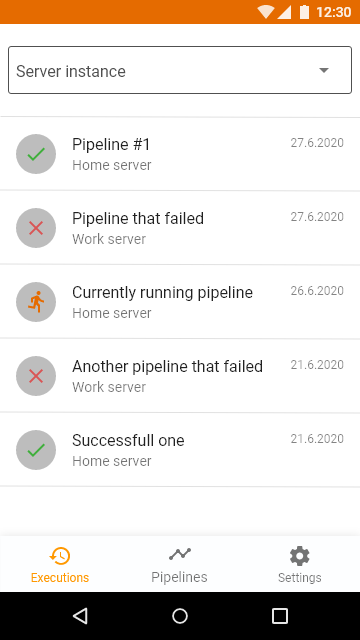
\includegraphics[width=\textwidth]{pics/xd/Bottom Navigation - executions.png}
    	\caption[History]{History screen design}\label{fig:xdHistory}
    \end{minipage}
    \begin{minipage}[b]{0.32\textwidth}
    	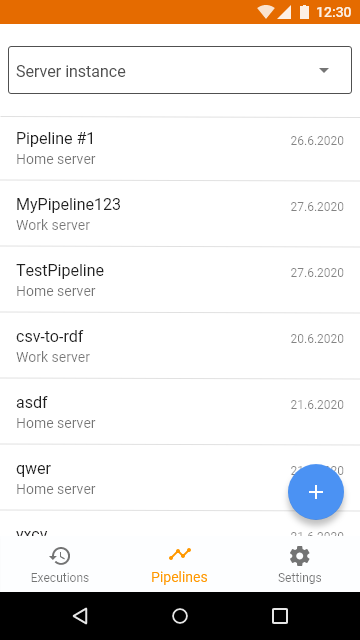
\includegraphics[width=\textwidth]{pics/xd/Bottom Navigation - pipelines.png}
    	\caption[Pipelines]{Pipelines screen design}\label{fig:xdPipelines}
    \end{minipage}
    \begin{minipage}[b]{0.32\textwidth}
    	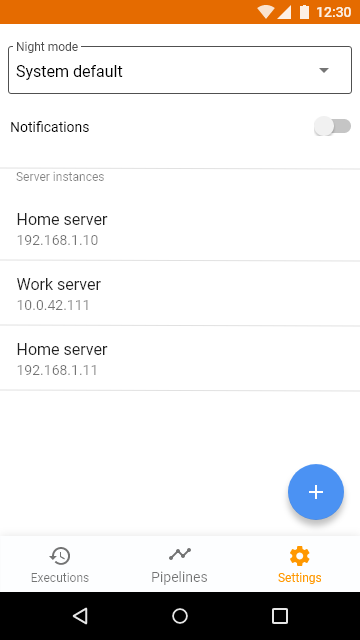
\includegraphics[width=\textwidth]{pics/xd/Bottom Navigation - settings.png}
    	\caption[Settings]{Settings screen design}\label{fig:xdSettings}
    \end{minipage}
\end{figure}

\subsection{Lists}
Each of the three main screens will display some sort of list.
For execution screen it's a list of executions, for pipeline screen it's a list of pipelines and for settings screen it's a list of server instances.

All of those lists will have one thing in common and that being the swipe gesture.
When users swipe an item to the left or to the right, the item will be deleted.
Users will have the ability to undo this operation for a short period of time.

Tapping on item from the pipeline screen will open the edit pipeline screen.
Long click on item from execution screen or from pipeline screen will launch the pipeline.

\begin{figure}\centering
    \begin{minipage}[b]{0.32\textwidth}
    	\includegraphics[width=\textwidth]{pics/xd/Bottom Navigation - pipelines – 1.png}
    	\caption[Deleting pipeline]{Deleting pipeline design}\label{fig:xdDeletePipeline}
    \end{minipage}
    \begin{minipage}[b]{0.32\textwidth}
    	\includegraphics[width=\textwidth]{pics/xd/Bottom Navigation - pipelines – 2.png}
    	\caption[Undo option]{Undo option design}\label{fig:xdUndo}
    \end{minipage}
\end{figure}

\section{Other screens}
\todo[inline]{another screen or other screens}
The three main screens are not the only screens our application will consists of.

\subsection{Edit server instance}
While registering new server instance or editing an already registered one, the application needs the address for communication and some name for labeling and better organising.
Users will be able to add a description of the instance, so that there is no pressure to store every information about the instance in the server name.
There could also be an option to ping the server (F-2.6, \autoref{subsec:ping}) to verify the address and a way to cancel the registration/edit.
Because of this, another screen, just for registering/editing server instances, will be added.

\begin{figure}\centering
    \begin{minipage}[b]{0.32\textwidth}
    	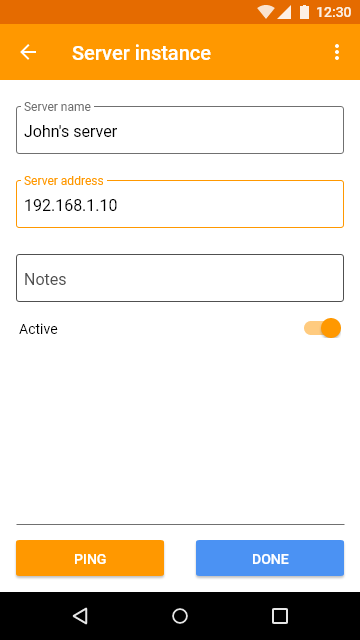
\includegraphics[width=\textwidth]{pics/xd/Edit server instance.png}
    	\caption[Edit server instance]{Edit server instance screen design}\label{fig:xdEditServerInstance}
    \end{minipage}
\end{figure}

\subsection{Edit pipeline screen}
According to the F-4.2 requirement, described in \autoref{subsec:editpipelinescreen}, there have to be a screen for editing pipelines.
This screen will be displaying pipeline components and drawing links between them.

\begin{figure}\centering
    \begin{minipage}[b]{0.32\textwidth}
    	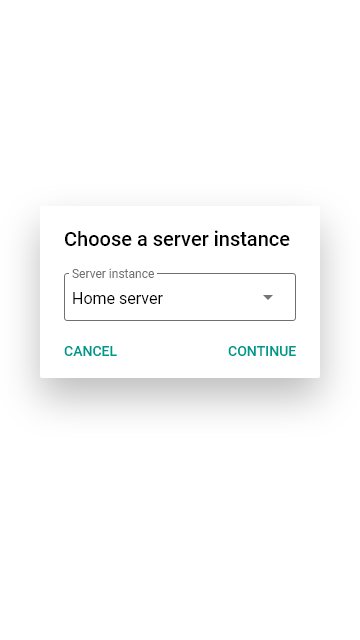
\includegraphics[width=\textwidth]{pics/xd/Create new pipeline.png}
    	\caption[Create new pipeline dialog]{Create new pipeline dialog design}\label{fig:xdCreateNewPipelineDialog}
    \end{minipage}
    \begin{minipage}[b]{0.32\textwidth}
    	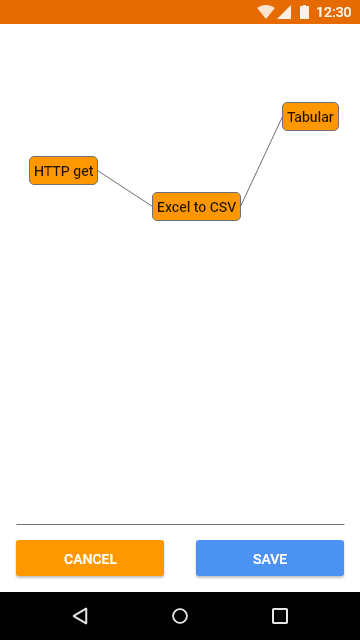
\includegraphics[width=\textwidth]{pics/xd/Pipeline editor.png}
    	\caption[Edit pipeline screen]{Edit pipeline screen design}\label{fig:xdPipelineEditor}
    \end{minipage}
\end{figure}

\subsection{Edit component screen}
This screen has to be created, because each pipeline's component has it's own settings.

\begin{figure}\centering
    \begin{minipage}[b]{0.32\textwidth}
    	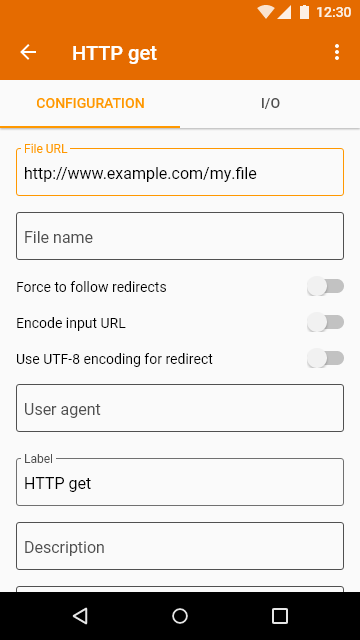
\includegraphics[width=\textwidth]{pics/xd/Edit component - configuration.png}
    	\caption[Edit component screen 1]{Edit component screen 1 design}\label{fig:xdEditComponent1}
    \end{minipage}
    \begin{minipage}[b]{0.32\textwidth}
    	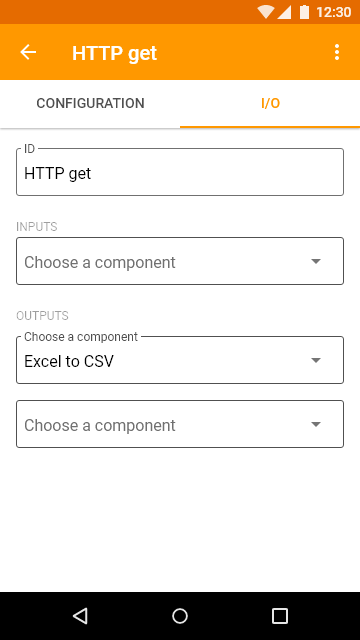
\includegraphics[width=\textwidth]{pics/xd/Edit component - io.png}
    	\caption[Edit component screen 2]{Edit component screen 2 design}\label{fig:xdEditComponent2}
    \end{minipage}
\end{figure}

\subsection{Notifications}
According to the F-3.1 requirement, described in \autoref{subsec:notifications}, notifications need to be implemented.

\begin{figure}\centering
    \begin{minipage}[b]{0.7\textwidth}
    	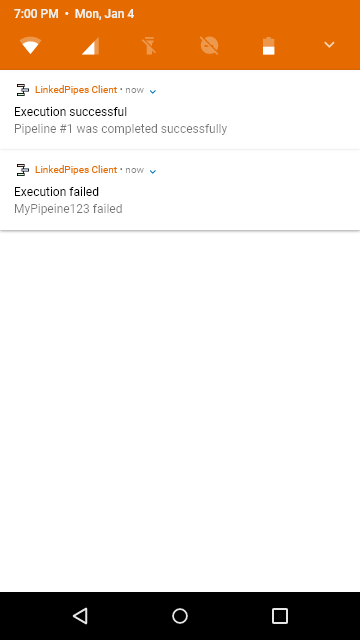
\includegraphics[width=\textwidth]{pics/xd/Notifications.png}
    	\caption[Notifications]{Notification design}\label{fig:xdNotifications}
    \end{minipage}
\end{figure}